
\label{sec:crosscutting}

% Drawn by scripts/revision3/fig_appendix_schematics.py; the .pptx is the
% editable source and is released with the paper.
\begin{figure*}[t]
\centering
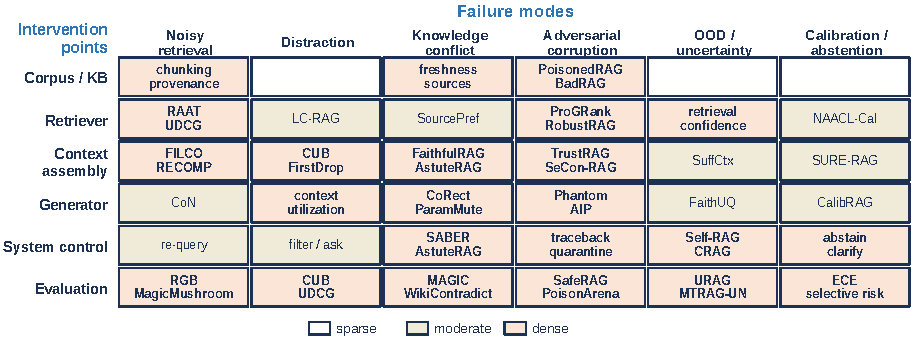
\includegraphics[width=\textwidth]{figures/generated/fig_failure_matrix.pdf}%
\caption{Schematic literature-family $\times$ intervention matrix. Shading and
example labels are illustrative design aids, not counts from Map~B;
quantitative Map-B distributions appear in Table~\ref{tab:corpus-stats}. Rows
are coordinate C3 and columns are coordinate C1, which is why a cell, not a
column, is the unit at which two systems become comparable.}
\label{fig:failure-intervention-matrix}
\end{figure*}

\begin{table*}[t]
\centering
\scriptsize
\renewcommand{\arraystretch}{0.92}
\begin{tabularx}{\linewidth}{>{\raggedright\arraybackslash}p{0.13\linewidth}>{\raggedright\arraybackslash}p{0.12\linewidth}>{\raggedright\arraybackslash}p{0.16\linewidth}>{\raggedright\arraybackslash}p{0.18\linewidth}>{\raggedright\arraybackslash}p{0.13\linewidth}>{\raggedright\arraybackslash}X}
\toprule
\textbf{Work} & \textbf{Failure} & \textbf{Task / setup} & \textbf{Key assumption} & \textbf{Metric} & \textbf{Boundary} \\
\midrule
IrrelCtx & irrelevant context & Open-domain QA & Irrelevance can be filtered or learned against & Robust accuracy & No adversarial/conflict setting. \\
RAAT & retrieval noise & Noisy QA training & Noise-aware training improves generation & F1/EM & Needs deployment-like noise. \\
RGB & multi-ability RAG & Bilingual benchmark & RAG reliability decomposes into abilities & Ability accuracy & Not adversarially adaptive. \\
FaithfulRAG & conflict & Fact-level conflict & Conflicts can be localised and reasoned over & Faithfulness & Needs reliable fact extraction. \\
AstuteRAG & imperfect retrieval & Training-free consolidation & Internal/external knowledge can be reliability-compared & Robust QA & Depends on LLM self-assessment. \\
PoisonedRAG & poisoning & Injected passages & Few crafted passages can dominate retrieval & Attack success & Targeted corruption focus. \\
RobustRAG & defense & Bounded corruption & Isolate-and-aggregate can certify robustness & Certificate, accuracy & Assumes attack budget. \\
Self-RAG / CtrlA & adaptive retrieval & Retrieve-or-answer & Model state can trigger retrieval & Trigger quality & Calibration can shift. \\
CalibRAG / URAG & calibration & Decision/MCQA & Confidence should reflect evidence uncertainty & ECE, coverage & Does not repair evidence. \\
PoisonArena / SafeRAG & security eval. & Poisoning benchmark & Threat models must be explicit & ASR, bypass & Still isolates attacks. \\
\bottomrule
\end{tabularx}
\caption{Analytical matrix of representative robust RAG work. Compared with a citation list, the matrix highlights each work's task setup, central assumption, metric focus, and boundary of applicability.}
\label{tab:analytical-matrix}
\end{table*}

\begin{table*}[t]
\centering
\scriptsize
\renewcommand{\arraystretch}{0.86}
\begin{tabularx}{\linewidth}{>{\raggedright\arraybackslash}p{0.13\linewidth}>{\raggedright\arraybackslash}p{0.17\linewidth}>{\raggedright\arraybackslash}p{0.17\linewidth}>{\raggedright\arraybackslash}p{0.16\linewidth}>{\raggedright\arraybackslash}p{0.13\linewidth}X}
\toprule
\textbf{Work} & \textbf{System setup} & \textbf{Failure construction} & \textbf{Metric / cost} & \textbf{Main claim} & \textbf{Failure boundary} \\
\midrule
IrrelCtx & RALM / open-domain QA; retrieved context injected into generator & Irrelevant passages with varying plausibility & Robust accuracy / answer degradation & Models can be brittle to irrelevant context. & Does not cover adversarial corruption or answerability policy. \\
RAAT & Noise-aware training for retrieval-augmented LMs & Multiple retrieval-noise types during training/evaluation & EM/F1 under noisy retrieval & Adaptive adversarial training improves noise robustness. & Transfer depends on whether deployment noise matches training noise. \\
RGB & Benchmark over English/Chinese QA-style RAG tasks & Noise, negative rejection, integration, counterfactual evidence & Ability-specific accuracy & RAG reliability decomposes into distinct abilities. & Benchmark abilities are diagnostic but not a unified control policy. \\
Sufficient Context & QA contexts labeled by sufficiency & Insufficient vs sufficient retrieved evidence & Selective answering / abstention quality & Evidence sufficiency should govern answerability. & Does not repair retrieval and does not model adversarial evidence. \\
PoisonedRAG & Corpus-injection attack against RAG & Crafted poisoned passages inserted into retrieval corpus & Attack success, retrieval of poison & Few poisoned documents can steer answers. & Strength depends on corpus write access, topic targeting, and retrieval success. \\
Certified / isolate defenses & Bounded-corruption RAG defense setting & Assumed corruption budget over retrieved evidence & Certificate, robust accuracy & Aggregation can certify robustness under budget assumptions. & Guarantees narrow when attacker violates budget or attacks instructions/tools. \\
Self-RAG / CtrlA & Adaptive retrieve-or-answer policies & Uncertainty about whether retrieval is needed & Trigger quality, answer utility, cost & Retrieval should be a conditional action. & Calibration shifts under distribution change; action cost often underreported. \\
RAGTruth & Annotated hallucination/faithfulness resource & Naturally generated unsupported spans across tasks & Span-level hallucination labels & Fine-grained support labels improve evaluation. & Faithfulness labels do not fully specify retrieval failure or system action. \\
\bottomrule
\end{tabularx}
\caption{Method-level comparison of representative robust-RAG work. The table makes explicit the setup, failure construction, metric target, main claim, and failure boundary that must be aligned before comparing methods.}
\label{tab:method-level-comparison}
\end{table*}


\begin{table*}[t]
\centering
\scriptsize
\renewcommand{\arraystretch}{0.86}
\begin{tabularx}{\linewidth}{>{\raggedright\arraybackslash}p{0.14\linewidth}>{\raggedright\arraybackslash}p{0.19\linewidth}>{\raggedright\arraybackslash}p{0.24\linewidth}>{\raggedright\arraybackslash}p{0.18\linewidth}X}
\toprule
\textbf{Case} & \textbf{Released rows / papers} & \textbf{Audited comparison fields} & \textbf{Metric or failure conflict} & \textbf{Synthesis / artifact boundary} \\
\midrule
Noise / distraction robustness & 5 rows: IrrelCtx, RAAT, Chain-of-Note, Sufficient Context, RGB & Assumption, QA dataset or benchmark slice, generator / reader setup, negative type, rank and gold-evidence availability. & EM/F1, rejection, selective risk, and ability-specific benchmark scores answer different questions. & Treat filtering, noise-aware training, generator reading, sufficiency prediction, and benchmark diagnosis as different mechanisms; artifact status is recorded per paper in the released worksheet. \\
Faithfulness, conflict, and attribution & 5 rows: RAGTruth, FaithfulRAG, AstuteRAG, Tug-of-War, Chain-of-Note & Unit of support, source-conflict assumption, attribution granularity, model-side reasoning setup, artifact availability. & Span-level support, fact-level conflict resolution, source preference, and final answer accuracy can disagree. & Citation faithfulness should not be collapsed into conflict robustness; the worksheet records where artifact evidence is dataset-level, code-level, or paper-only. \\
Adversarial corruption and RAG security & 6 rows: PoisonedRAG, corpus poisoning, BadRAG, certified defense, TrojanRAG, traceback & Corpus write access, insertion budget, retriever visibility, query control, generator access, stealth, retrieved malicious evidence, defense timing. & Attack success, certified robust accuracy, detection, traceback, and clean utility are not one defense score. & Compare only inside a capability envelope; prevention, demotion, detection, traceback, recovery, and certification remain separate outcomes. \\
Calibration, abstention, and adaptive control & 5 rows: Sufficient Context, Self-RAG, CRAG, CalibRAG, uncertainty RAG & Confidence target, evidence sufficiency labels, retrieval trigger, action set, cost budget, model/policy setup. & ECE, selective risk, coverage, retrieval-trigger quality, and answer utility can move in different directions. & Separate belief estimation from action selection; report coverage, cost, and final action alongside correctness. \\
Evaluation and benchmark comparability & 5 rows: RGB, RAGTruth, Sufficient Context, query robustness, RAG security benchmark & Evidence-state labels, perturbation source, model outputs scored, threat model, benchmark artifact availability. & Harder scores may reflect retrieval instability, unsupported spans, unanswerability, or adversarial steering. & Evaluation resources are diagnostic slices, not a universal robustness scale; benchmark comparisons require aligned evidence state and action policy. \\
\bottomrule
\end{tabularx}
\caption{Deeper case-study synthesis. The released 26-row worksheet compares assumptions, datasets or benchmark settings, model/evidence setup, metrics, failure modes, artifact availability, and comparison implications for the same five C1--C5 cases.}
\label{tab:deep-case-study-matrix}
\end{table*}

\begin{table*}[t]
\centering
\scriptsize
\renewcommand{\arraystretch}{0.9}
\begin{tabularx}{\linewidth}{>{\raggedright\arraybackslash}p{0.19\linewidth}>{\raggedright\arraybackslash}p{0.24\linewidth}>{\raggedright\arraybackslash}p{0.23\linewidth}X}
\toprule
\textbf{Apparent conclusion} & \textbf{What the framework changes} & \textbf{Non-trivial finding} & \textbf{Implication} \\
\midrule
``Method A is more robust to noise than method B.'' & Aligns noise type, rank position, gold-evidence availability, and intervention point. & Some methods solve generator distraction while others solve retriever defects; their scores are not competing estimates of the same property. & Report noise source and intervention point before ranking methods. \\
``Defense X lowers attack success.'' & Separates prevention, demotion, detection, traceback, and recovery. & A defense can improve traceback without lowering user-facing attack success, or certify bounded corruption without handling prompt-bearing documents. & Security papers should report outcome type, not only attack success rate. \\
``Calibration improves reliability.'' & Separates confidence in answer correctness from evidence sufficiency and action utility. & A calibrated answerer can still answer from insufficient evidence; an abstaining system can lower risk while reducing coverage. & Calibration metrics should be paired with evidence and action metrics. \\
``Benchmark Y is harder.'' & Compares evidence state, required action, cost budget, and metric target. & A benchmark can be hard because retrieval fails, because evidence conflicts, or because the correct action is refusal; these failures should not be pooled. & Leaderboards should expose diagnostic sub-scores instead of one robust-RAG score. \\
\bottomrule
\end{tabularx}
\caption{Distilled classes of non-trivial findings produced by the comparability framework. Main Table~\ref{tab:main-normalization-findings} gives the concrete paper-pair cases; this appendix table groups them into reusable interpretation rules.}
\label{tab:nontrivial-findings}
\end{table*}

\begin{table*}[t]
\centering
\scriptsize
\renewcommand{\arraystretch}{0.9}
\begin{tabularx}{\linewidth}{>{\raggedright\arraybackslash}p{0.24\linewidth}>{\raggedright\arraybackslash}p{0.25\linewidth}>{\raggedright\arraybackslash}p{0.21\linewidth}X}
\toprule
\textbf{Main claim} & \textbf{Cited evidence basis} & \textbf{What the evidence supports} & \textbf{Boundary} \\
\midrule
Irrelevant or noisy context can harm generation. & Irrelevant-context robustness, RAAT, RGB, and counterfactual-noise studies. & Noise affects both retrieval quality and generator context use. & Does not imply one robustness score covers all noise types. \\
Knowledge conflict differs from adversarial corruption. & Conflict and poisoning studies with different evidence origins and evaluation targets. & Natural disagreement and attacker-created contradiction require different assumptions. & Conflict-resolution results should not be read as poisoning-defense results. \\
RAG attacks require capability normalisation. & Poisoning, backdoor, prompt-injection, traceback, and certification studies. & Attack/defense results require corpus access, query control, retriever visibility, and budget. & The paper does not rank attacks by real-world prevalence. \\
Calibration, abstention, and retrieval control are distinct. & Sufficient-context, uncertainty, adaptive-retrieval, and calibration studies. & Confidence estimation, evidence sufficiency, retrieval triggering, and abstention optimise different quantities. & Does not validate a single universal control policy. \\
Action-trace evaluation is a benchmark agenda. & Benchmarks exposing subsets of answer, evidence, action, cost, and threat fields. & Existing benchmarks cover pieces of the proposed schema. & No new leaderboard or empirical system ranking is claimed. \\
\bottomrule
\end{tabularx}
\caption{Narrative claim-to-source ledger. Expanded and strict citation audits
were model-assisted and deterministic; this table records the intended evidence
boundary rather than certifying every citation.}
\label{tab:claim-verification-ledger}
\end{table*}


\subsection{Peer-Reviewed Backbone and Preprint Trends}

The main synthesis is anchored in the venue-linked backbone summarised in Table~\ref{tab:peer-reviewed-backbone}. Under that stricter evidence stratum, five conclusions remain stable: retrieved evidence can harm generation; conflict and poisoning require different assumptions; security results require attacker-capability normalisation; calibration and abstention are separate control decisions; and answer accuracy alone is insufficient for robust-RAG evaluation. The broader 268-paper adjudicated map is still useful, but mainly for trend discovery and auditability. Its preprint-heavy cross-tabs are moved to Appendix~\ref{sec:map-statistics}; they diagnose where the map is dense or sparse, but they are not used as field-wide prevalence estimates.

\paragraph{Critical judgments from the re-analysis.}
The framework weakens three common readings of the literature. First, many ``robust to retrieval noise'' claims are over-broad: once distractor hardness, gold-evidence availability, and intervention point are aligned, several methods address complementary mechanisms rather than competing on one robustness axis. Second, many RAG security defenses are narrower than their abstracts suggest: a defense against bounded factual corruption is not evidence of robustness to prompt-bearing documents, trigger-based backdoors, or post-hoc traceback settings. Third, answer-only benchmark gains are often under-specified: without citation support, evidence sufficiency, and action-cost labels, a higher score can mean better answering, riskier coverage, or simply more computation. These are the places where the framework changes interpretation rather than merely renaming categories.

\subsection{Where Robustness Interventions Act}

Across the literature, robustness interventions cluster by where they act in the RAG pipeline. \textbf{Corpus-level interventions} sanitise, filter, watermark, or validate documents before indexing. They are attractive because they prevent bad evidence from entering the system, but they require corpus governance and may not be possible for open-web retrieval. \textbf{Retriever-level interventions} improve ranking, detect poisoned passages, or diversify evidence. They are efficient and model-agnostic, but they only control what enters the context, not how the generator uses it. \textbf{Context-level interventions} compress, reorder, or filter the retrieved context. They are flexible, but can remove qualifiers or multi-hop evidence. \textbf{Generator-level interventions} use prompting, fine-tuning, note-taking, self-reflection, or hidden-state control. They directly address evidence use but may be model-specific. \textbf{System-level interventions} decide when to retrieve, verify, abstain, or ask. They are closest to deployment needs but require calibrated signals from all earlier stages.

This intervention map helps explain why papers sometimes appear to solve the same problem while actually operating at different layers. For example, irrelevant-context filtering \citep{irrelevantContext2023}, Chain-of-Note \citep{chainOfNote2023}, and Sufficient Context \citep{sufficientContext2024} all address unreliable evidence, but the first filters evidence, the second changes generator reasoning, and the third changes answer policy. Similarly, PoisonedRAG-style attacks \citep{poisonedRAG2024} target the corpus-to-generation path, while AIP attacks prompt templates \citep{aip2025}. A comprehensive survey must therefore compare methods by intervention point, not only by reported task accuracy.

\subsection{Critical Case Studies of Taxonomy Use}
\begin{table*}[t]
\centering
\scriptsize
\renewcommand{\arraystretch}{0.9}
\begin{tabularx}{\linewidth}{>{\raggedright\arraybackslash}p{0.17\linewidth}>{\raggedright\arraybackslash}p{0.25\linewidth}>{\raggedright\arraybackslash}p{0.25\linewidth}X}
\toprule
\textbf{Case} & \textbf{Papers / settings compared} & \textbf{Why naive comparison fails} & \textbf{Synthesis from the framework} \\
\midrule
Noise / distraction robustness & IrrelCtx, RAAT, RGB, Chain-of-Note, Sufficient Context & Some vary retriever noise, some change generator reading behavior, and some decide answerability; robust accuracy, ability scores, and abstention metrics answer different questions. & Treat retrieval imperfection, harmful context influence, and insufficient evidence as separate states; compare methods only after fixing the intervention point and required action. \\
Faithfulness, conflict, and attribution & RAGTruth, FaithfulRAG, AstuteRAG, Tug-of-War, Chain-of-Note & Span-level support, fact-level conflict, document-level reading, and final answer correctness are different target objects. & Citation faithfulness is not the same as conflict robustness; valid comparisons must state support unit, source reliability assumption, and action policy. \\
Adversarial corruption and RAG security & PoisonedRAG, BadRAG, certified defenses, traceback methods, prompt-injection defenses & One result may assume corpus write access, another bounded corruptions, another instruction-bearing documents, and another post-hoc observability; attack success rates transfer poorly across assumptions. & Report corpus write access, insertion budget, retriever visibility, generator access, stealth, and whether malicious evidence was retrieved before comparing attacks or defenses. \\
Calibration, abstention, and adaptive control & Self-RAG, CRAG, CalibRAG, uncertainty RAG, Sufficient Context & ECE, selective risk, retrieval-trigger quality, and abstention precision measure different objects; better confidence does not necessarily repair evidence or choose the right user action. & Separate belief estimation from action selection. A complete benchmark should score confidence, evidence sufficiency, final action, and cost. \\
Evaluation and benchmark comparability & RGB, RAGTruth, Sufficient Context, query-robustness benchmarks, RAG security arenas & A benchmark can be hard because retrieval fails, evidence conflicts, attribution is unsupported, the item is unanswerable, or an attacker is stronger. & Evaluation resources should expose diagnostic sub-scores and threat/action labels rather than one robust-RAG scalar. \\
\bottomrule
\end{tabularx}
\caption{Critical case studies showing how the comparability framework changes interpretation of representative robust-RAG papers.}
\label{tab:critical-case-studies}
\end{table*}


\paragraph{Case 1: irrelevant evidence is not one problem.}
IrrelCtx, RAAT, RGB, Chain-of-Note, and Sufficient Context are sometimes all described as robustness-to-noise work, but they instantiate different experimental objects. IrrelCtx tests whether a generator can ignore irrelevant context; RAAT treats noise as a training distribution; RGB decomposes reliability into benchmark abilities; Chain-of-Note changes the generator's intermediate reading behavior; Sufficient Context changes the answer policy when evidence is inadequate. A direct leaderboard comparison would mix retrieval perturbation, generator selectivity, and answerability control. The taxonomy changes the question from ``which method is best under noise?'' to ``which evidence state is present, which module intervenes, and what action should be scored?''

\paragraph{Case 2: poisoning papers differ by attacker capability.}
Poisoning Retrieval Corpora, PoisonedRAG, BadRAG, TrojanRAG, Phantom, AIP, and newer one-shot or traceback studies are all adversarial, but they assume different access and objectives. Some manipulate dense retrieval, some steer final answers, some rely on triggers, some attack shared prompt templates, and some evaluate whether poisoned evidence can be traced after the fact. Attack success rate is therefore not a portable metric unless corpus write access, query control, retriever visibility, generator access, insertion budget, and stealth requirements are aligned. This is why Table~\ref{tab:attacker-capability} treats capability fields as part of the result, not just implementation detail.

\paragraph{Case 3: calibration is not the same as abstention.}
UncertaintyRAG, CalibRAG, URAG, Self-RAG, CtrlA, Sufficient Context, and SABER-style trust/abstain methods all relate to uncertainty, but they optimise different objects. Some estimate uncertainty in spans or answer sets; some calibrate decision confidence; some decide when to retrieve; some decide when to abstain; some predict whether the retrieved context is sufficient. Expected calibration error, selective risk, retrieval-trigger accuracy, and abstention precision cannot be collapsed into one number. The taxonomy forces a distinction between belief estimation and action selection, explaining why a method can improve calibration without repairing evidence or improve retrieval triggering without improving final answer faithfulness.

\paragraph{Case 4: poisoning defenses do not share one threat model.}
Certified defenses, isolate-and-aggregate defenses, poisoned-document detectors, activation-based traceback, and prompt-injection defenses respond to different adversarial assumptions. A certificate can be meaningful under a bounded corruption budget but irrelevant when the attacker controls prompt-like instructions; a traceback method may be useful after an incident but may not prevent answer steering; a prompt-injection defense may not address embedding-space poisoning. The framework therefore asks defense papers to report the same capability fields as attack papers and to distinguish prevention, detection, demotion, traceback, and recovery.

\subsection{Strengths and Weaknesses by Method Family}

Filtering and reranking are attractive robustness methods because they can be added around existing LLMs. Their weakness is false negatives: an aggressive filter may discard the only passage that supports a rare or multi-hop answer. Robust training can teach models to ignore noise, but training data may not cover future attacks or domain-specific distractors. Conflict modeling provides a principled way to handle contradictions, but fact extraction and alignment remain brittle for long, compositional, or numerical claims. Certified defenses provide valuable guarantees, but their assumptions are often narrower than realistic attack surfaces. Adaptive retrieval and abstention improve risk control, but their performance depends on calibration signals that can themselves be miscalibrated under distribution shift.

The synthesis suggests that method families should be composed according to risk profile rather than stacked indiscriminately. A low-risk FAQ system may only justify lightweight filtering and citation checks, while a high-stakes document-grounded setting may require source validation, contradiction detection, selective abstention, and escalation. These are design implications, not claims that the evidence map validates any particular enterprise, medical, or legal deployment.

\subsection{What Counts as Progress?}

The corpus currently reports progress through heterogeneous metrics: EM/F1, hallucination rate, retrieval recall, attack success rate, calibration error, abstention accuracy, and human preference. These metrics are not directly comparable. A defense that reduces attack success may reduce answer utility; a calibration method may improve selective risk while lowering coverage; a retriever that improves recall may increase distraction. Robust RAG progress should therefore be reported as a Pareto frontier across utility, robustness, calibration, cost, and security. This mirrors the broader lesson from trustworthy ML: robustness is not a scalar property but a tradeoff surface.

\subsection{What Is Still Missing from the Literature}

Several gaps recur across categories. First, benchmarks rarely combine failures. Noise, conflict, poisoning, and unanswerability are usually tested separately, even though realistic systems may encounter them jointly. Second, many papers evaluate with one retriever and one generator, making transfer difficult to assess. Third, few works evaluate long-term corpus dynamics: documents are updated, poisoned documents are removed, indices are rebuilt, and user feedback changes future retrieval. Fourth, most papers treat users as passive recipients rather than interactive participants who can clarify intent or verify sources. Fifth, multilingual and multimodal robust RAG remains underdeveloped relative to text-only English QA; because our corpus is also text-heavy, this is a boundary of the present survey rather than a resolved conclusion about those areas.
